\section{Introduction}

Parkinson's disease (PD) is a common motor neurodegenerative disorder, characterized in part by the progressive loss of pigmented dopaminergic neurons from the \textit{Substantia Nigra pars compacta}. The main neuropathological hallmark of PD is the progressive accumulation of $\alpha$-synuclein in fibrillar aggregates named Lewy Bodies (in the soma) or Lewy Neurites (in neurites) \cite{Dehay_2015}. Interestingly, Lewy pathology follows a predictable pattern of progression in the brain suggesting that $\alpha$-synuclein can propagate from neurons to neurons \cite{Braak_2003}. Such observation, common to many neurodegenerative diseases \cite{Jucker_2018}, prompted initiatives to model and predict pathology progression in the brain of patients with neurodegenerative disorders. \\
\\
In 2012, Raj and colleagues developed a Network Diffusion Model (NDM) to predict atrophy progression in dementia \cite{Raj_2012}. For this purpose, they compared Magnetic Resonance Imaging recordings from healthy young subjects, healthy old subjects, and old patients suffering from either Frontotemporal Dementia or Alzheimer's Disease. Their study suggested that patterns of atrophy within the dementia spectrum could be explained by transmission of the disease along neuronal pathways. Using their model, they demonstrated a path for predicting future atrophy in individuals starting from baseline. The NDM model was later applied to other diseases using various kind of data. In 2017, Mezias and Raj showed that the spread of amyloid-$\beta$ pathology, involded in Alzheimer's disease, in mice was driven by spatial proximity but not network connectivity \cite{Mezias_2017_abeta}. At the opposite, progression of tau pathology, also involved in Alzheimer's disease and other tauopathies, was better recapitulated by connectivity \cite{Mezias_2017_tau}. In 2019, Henderson and colleagues reported that progression of $\alpha$-synuclein pathology, similary to tau pathology, is largely predicted by anatomical connectivity between brain structures \cite{Henderson_2019}. \\
\\
We here replicated the  core of the NDM applied to $\alpha$-synuclein spread in mice as implemented by Henderson and colleagues \cite{Henderson_2019}. Both R scripts, connectivity matrix and experimental datasets were made fully accessible by the authors on GitHub allowing an easy process. We were able to reproduce qualitatively and quantitatively the main results of the paper. The aim of the present replication is not to fully replicate the entire paper but to focus on the core model and main immediate results.\\
\\
\section{Background}
\subsection{Graph Theory and brain connectivity}
Henderson et al. combined quantitative pathology mapping in the mouse brain with network modeling to understand the spatiotemporal pattern of spread of  $\alpha$-synuclein pathology \cite{Henderson_2019}. Graph theory is a branch of mathematics applicable to Neuroscience. The brain is a complex system that can be modeled as a network or graph. When applied properly, Graph theory can offer important insights into different aspects of brain networks such as architecture, evolution, development, or clinical disorder \cite{Sporns_2018}.\\
\\
Networks are defined as a collection of elements (or nodes) and their pairwise links (or edges) that can be summarized in the form of a connectivity matrix (named adjacency matrix). Depending on the type of graph, edges can have binary values (present: 1 - absent: 0) or actual weights reflecting connection strength. A graph is called undirected when an edge $e$ reciprocally connects nodes $V_{a}$ and $V_{b}$. Conversely, a graph is named directed when the edge $e$ is projecting from $V_{a}$ to $V_{b}$ but not from $V_{b}$ to $V_{a}$.\\
\\
Thanks to the initiative from the Allen Institute for Brain Science's Mouse Connectivity Atlas (MCA), the mouse brain connectome is now freely accessible for the neuroscience community \cite{Oh_2014}. In a matrix, connectivity is represented as "outgoing" along  rows and "incoming" along  columns. From the adjacency matrix, the in-degree and out-degree distributions can be computed as respectively the sum of all entries in the corresponding row and the sum of all entries in the corresponding column and are represented in diagonal matrices.\\
\\
The Laplacian graph is a matrix used to explore the properties of a network. It is computed using the adjacency matrix and either the in-degree or out-degree graph depending on the applications.

\subsection{Model description}
The model used by Henderson et al. requires the mouse brain connectome (discussed in the previous section) and whole brain $\alpha$-synuclein pathology quantification.\\
\\
The model used in the study is the classical $\alpha$-synuclein pre-formed fibrils (PFFs -  5$\mu$g) unilateral injection in the dorsal striatum of non-transgenic mice (NTG) \cite{Luk_2012, Henderson_2019}. Following inoculation, NTG mice were terminated at 3, 6, or 9 months post-injection (MPI). Brain pathology was assessed using traditional immunohistochemical methods to detect pathological $\alpha$-synuclein phosphorylated on Serine129 (pS129). Quantification (as percent of region occupied by immunostaining) was performed on both brain hemispheres (ipsilaterally and contralaterally to the injection point) in 58 different regions. Thus, the pathology dataset provided by the authors on their repository is an Excel sheet with values for 5 mice per group and timepoint for all 116 brain regions.\\
\\
Using the dataset from \cite{Oh_2014} for synaptic connection, the authors generated a directed and weighed connectivity graph $G={V,E}$ whose nodes $V$ are $N$ cortical and subcortical grey matter regions and whose edges $e_{ij} \in E$ represent an axonal projection from $V_{i}$ to $V_{j}$. They then defined the weighed adjacency matrix of $G$ as $A = [A_{ij}]$ generating a final parcellation of 116 regions.\\
\\
The magnitude of observed $\alpha$-synuclein pathology of all $N$ nodes at a time $t$ is the vector $x_{t}$. The predicted regional $\alpha$-synuclein pathology $\widehat{x_{t}}$ is a function of the adjacency matrix $A$ and a seed region $seed$ ($\in E$)  and is computed as shown in (1):

\begin{equation}
    \widehat{x_{t}}=e^{-cLt} x_{o}
\end{equation} $\\$

Where:
\begin{itemize}
\item $c$ is a constant designed to achieve an optimal match with the data as the empirical diffusion constant for the pathology is \textit{a priori} unknown.
\item $t$ stands for the timepoint of the prediction. 
\item $L$ is the out-degree Laplacian matrix computed as shown in (2):

  \begin{equation}
    \begin{cases}
      -A_{ij} & \text{for $i \neq j$} \\
      \sum_{j=1}^N A_{ij} & \text{for $i=j$} \\
  \end{cases}
\end{equation}
\item  $x_{0}$ is the seed vector computed as shown in (3):
  
  \begin{equation}
    x_{0}
    \begin{cases}
        0 & \text{for $i \neq seed$} \\
        1 & \text{for $i = seed$} \\
    \end{cases}
  \end{equation}
\end{itemize}
   

\section{Material and Methods}
\subsection{Replication of the Model}
Henderson et al. coded their model using RStudio 3.3.3. Codes and data were made accessible on GitHub.A first folder available, contains the scripts that are specific to the analysis. A second one consists of the numerous data sets used in the study, notably, the pathology data set, the connectivity matrices, and the \textit{Snca} gene expression energy value data set.\\
\\
Using Python 3.7 and Windows 10 Operating System, we successfully replicated the scripts summarized in the \textbf{Table ~\ref{tab:table1}}. We also ran the scripts using Mac Operating System \textbf{ [version] } to look for inter-compatibility between Operating Systems.\\

\begin{table}[ht]
  \begin{center}
    \caption{\textbf{Scripts successfully replicated}}
    \label{tab:table1}
    \begin{tabular}{|l|c|r|} % <-- Alignments: 1st column left, 2nd middle and 3rd right, with vertical lines in between
      \hline
      \textbf{From Henderson et al.} & \textbf{Equivalent in Python} & \textbf{Function}\\

      \hline
      process$\_$pathconn.R & process$\_$files.py & Processes the input data sets\\
      getLout.R & Laplacian.py & Compute the out-degree\\
       &  & Laplacian matrix\\
      fitfxns.R $\rightarrow$ make.Xo & fitfunctions.py & Sets the seed of the model\\
      
      fitfxns.R $\rightarrow$ predict.Lout & fitfunctions.py & Predicts the pathology\\ 
      fitfxns.R $\rightarrow$ c.fit & fitfunctions.py & Obtains a c value that fits the\\
      & & model\\ 
      \hline

      
    \end{tabular}
  \end{center}
\end{table}
We replicated the core of Henderson et al. code and we subsequently were capable of computing the pathology prediction $\widehat{x}$(t) for the three different timepoints in NTG mice. We aimed at reproducing the main results of the original paper and we retrieves both qualitative and quantitative data observed by the authors.\\

\subsection{Pipeline of our code}

Our code consists of a main script named $pipeline.py$ made of a DataManager to easily change the different parameters such as the timepoints, the seed, or the quantified pathology matrix. $pipeline.py$ successively calls the scripts mentioned below and saves the data as tables and figures.\\
\\
$process$\_$files.py$ processes the data inputs (Quantified pathology matrix, ipsilateral connectivity matrix, and contralateral connectivity matrix). Its main outputs are the adjacency matrix, a pathology matrix, and the list of regions of interest shaped as panda DataFrames.\\
\\
$Laplacian.py$ computes, from the adjacency matrix, the out-degree Laplacian matrix. After careful observations, we successfully replicated the Laplacian matrix that captures the retrograde connectivity.\\
\\
$fitfunctions.py$ is a set of functions with different roles. $make$\_$Xo$ has been reproduced as described in Henderson's code. As mentioned before, $make$\_$Xo$ produces of a column vector (here shaped as a panda DataFrame) that contains 0 for non-seed regions or 1 for the seed region. $predict$\_$Lout$ predicts the regional $\alpha$-synuclein pathology when given the Laplacian, the seed, a timepoint of prediction, and the tuning constant c. $c$\_$fit$ returns the value of the best fit c and the best correlation coefficient using $predict$\_$Lout$ and Pearson's correlation test.\\
\\
The pipeline also runs different scripts that we used for our own study (stability of the model, robustness, comparison with an iterative model). More information on how to use our code and the requirement related to the inputs can be encountered in the ReadMe section available in our corresponding GitHub repository. \textbf{Add an hyperlink when done}\\

\section{Results}
\subsection{Network model of pathological $\alpha$-synuclein spread}
The network diffusion model validated by Henderson et al. is based on anatomical connectivity. Using this model, their team estimated pathology as a function of time given the introduction of misfolded $\alpha$-synuclein into the ipsilateral Caudoputamen (iCPu).\\
\\
\textbf{Figure~\ref{fig:fig1}.A-C} illustrate the correlation between our predicted data and the quantified data. We appreciated a visual consistency between our Scatterplots and those displayed by Henderson and colleagues. We could also extract the same Pearson's r scores (0.56, 0.69 and 0.65 with respect to the MPI 1, the MPI 3, and the MPI 6).\\
\\
Finally, our model also computes p-values that are equal to those from the original paper before and after Bonferroni correction. \textbf{Table ~\ref{tab:table2}} summarizes these results.
These data suggests that linear dynamics imposed on a connectivity network can explain pathology spread over time.\\

\begin{table}[ht]
  \begin{center}
    \centering
    \caption{\textbf{Data correspondence between the reproduced results and the original article}$\newline$ The results have been rounded up to the third decimal.}
    \label{tab:table2}
    
    \begin{tabular}{|l|c|c|} % <-- Alignments: 1st column left, 2nd middle and 3rd middle, with vertical lines in between
      \hline
      
      &\textbf{Henderson et al.} & \textbf{Our Model} \hspace{1cm}\\

      \hline
      Best constant c computed & $1.625$ & $1.625$ \\
      MPI 1 & &\\
            \hspace{1cm} p-value before Bonferroni & $2.695e^{-9}$ & $2.695e^{-9}$ \\ 
            \hspace{1cm} correction & &\\
            \hspace{1cm} p-value after Bonferroni & $8.085e^{-9}$ & $8.085e^{-9}$ \\ 
            \hspace{1cm} correction & &\\
            \hspace{1cm} correlation R & $0.559$ & $0.559$\\
      MPI 3& &\\
            \hspace{1cm} p-value before Bonferroni & $<$ $2.2e^{-11}$ & $1.150e^{-17}$ \\ 
            \hspace{1cm} correction & &\\
            \hspace{1cm} p-value after Bonferroni & $3.451e^{-17}$ &  $3.451e^{-17}$ \\ 
            \hspace{1cm} correction & &\\
            \hspace{1cm} correlation R & $0.696$ & $0.696$ \\
      
      MPI6& &\\
            \hspace{1cm} p-value before Bonferroni & $8.793e^{-15}$ & $8.793e^{-15}$ \\ 
            \hspace{1cm} correction & &\\
            \hspace{1cm} p-value after Bonferroni & $2.638e^{-14}$& $2.638e^{-14}$ \\ 
            \hspace{1cm} correction & &\\
            \hspace{1cm} correlation R & $0.648$ & $0.648$ \\
      \hline

      
    \end{tabular}
  \end{center}
\end{table}

Then, we imposed some controls on on our model to assess its robustness. As performed in the original article, we randomly seeded the diffusion model and plotted the fit r for each timepoint. \textbf{(Figure ~\ref{fig:fig1}.D)} This revealed that CPu seed produces either the best fit (3 MPI and 6 MPI) or the second-best fit (1 MPI) as observed by Henderson et al. as well. 
Likewise as published in 2017 by Pandya et al., we randomly shuffled the connectivity matrix \textbf{(Figure ~\ref{fig:fig1}.E)} and the pathology matrix \textbf{(Figure ~\ref{fig:fig1}.F)}. For each shuffle, we plotted the corresponding fit. \cite{Pandya_2017} Our results confirm that the spatiotemporal spread is indeed driven by connectivity.


\begin{figure}[h]
 
    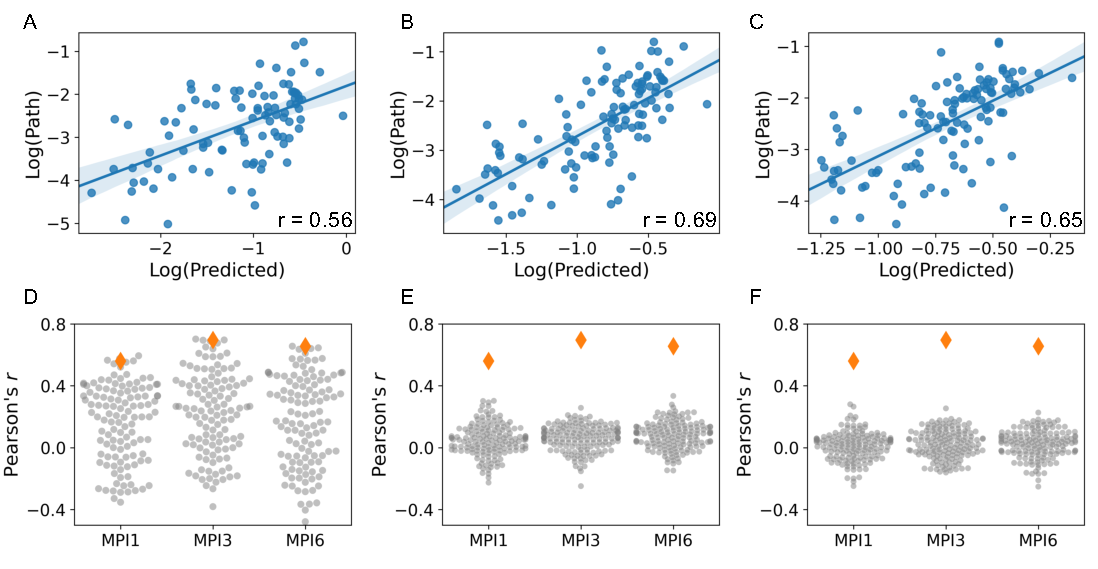
\includegraphics[width = \linewidth]{Figures/Fig1.pdf}
    \centering
    \caption{\textbf{Network diffusion model based on anatomical connectivity explains pathological $\alpha$-synuclein spread}\\
    \label{fig:fig1}
    Scatterplots and Pearson's correlation coefficient (r) of log(predicted) pathology based on anatomical connectivity versus actual log(pathology) values. Predictions versus pathology are shown 1 month (\textbf{A}), 3 month (\textbf{B}) or 6 month (\textbf{C}) after injection of PFF (5$\mu$g) into the ipsilateral CPu.
    \textbf{D}, Different brain regions were used as seed and pathology was modeled from each site. The fit for one specific seed was plotted and we reiterated the experiment for each timepoint. The red dot represents the fit obtained when the model is seeded into the iCPu. \textbf{E}, The pathology matrix was randomly shuffled and the fit was subsequently computed for each timepoint. The red dot represents the fit obtained when the model is seeded into the iCPu and the pathology matrix is not randomly shuffled. \textbf{F}, The connectivity matrix was randomly shuffled and the fit was subsequently computed for each timepoint. The red dot represents the fit obtained when the model is seeded into the iCPu and the adjacency matrix is not randomly shuffled.}
    
\end{figure}
    
\subsection{Differential vulnerability of regions is correlated with $\alpha$-synuclein expression}
As intrinsic vulnerability had been hypothesized to be a critical factor in the development of pathology, Henderson et al. thought to investigate that aspect using the connectivity-based model. They defined the difference between predicted pathology and observed pathology as a measure of relative vulnerability. Regions with greater values or lower values compared to the predicted data are considered respectively as relatively vulnerable or resilient regions. In \textbf{Figure ~\ref{fig:fig2}.A} we replicated the areas of relative vulnerability as those inferred by Henderson et al.\\
\\
To determine whether the prediction could be improved, Henderson et al. seek out for factors that would explain regional vulnerability. They postulated that \textit{Snca} gene expression should influence the development of the pathology. Using \textit{Snca} expression energy values obtained from the Allen Brain Atlas, it was possible to investigate the relationship between \textit{Snca} gene expression and regional vulnerability. \textbf{Figure ~\ref{fig:fig2}.B} illustrate the \textit{Snca} Expression energy values in different sections of the brain. In support with their hypothesis, \textit{Snca} expression was highly correlated with vulnerability values. Both Figure A and B are displayed using the Python package Brainrender. \cite{Claudi_2021}
\\
\begin{figure}

    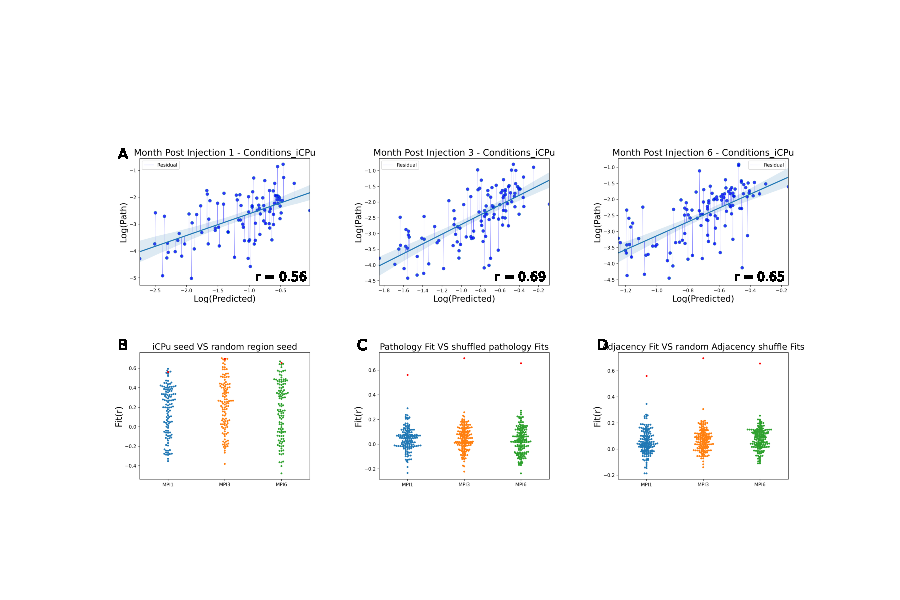
\includegraphics[width= \linewidth]{Figures/Fig2.pdf}
    \centering
    \caption{\textbf{Differential vulnerability of regions is correlated with $\alpha$-synuclein expression} \\
    \label{fig:fig2}
    \textbf{A}, Heatmap of the residuals between the log(predicted) and log(pathology) are plotted on an anatomical mouse brain as a measure of the relative vulnerability of regions after prediction of the MPI 1.
    \textbf{B}, Heat map of the SNCA mean expression energy values from the Allen Brain Atlas in situ hybridization for each of the designated region.
    Both Figure A and B are displayed using the Python package \textit{Brainrender}. \cite{Claudi_2021}}
\end{figure}
    
Incorporation of \textit{Snca} expression into the network diffusion model was performed by weighting the outgoing connections of every node by its respective \textit{Snca} expression value. \textbf{Figure ~\ref{fig:fig3}} is a replication of the model using the data from Henderson et al GitHub repository. Taken all together, these data suggest that \textit{Snca} gene expression is an important factor impacting the vulnerability of regions and subsequently pathology spread. \textbf{Table~\ref{tab:table3}} displays a data correspondence between the reproduced results and the original article.

\begin{table}[ht]
  \begin{center}
    \centering
    \caption{\textbf{Data correspondence between the reproduced results and the original article after incorporation of the \textit{Snca} expression}$\newline$ The results have been rounded up to the third decimal.}
    \label{tab:table3}
    
    \begin{tabular}{|l|c|c|} % <-- Alignments: 1st column left, 2nd middle and 3rd middle, with vertical lines in between
      \hline
      
      &\textbf{Henderson et al.} & \textbf{Our Model} \hspace{1cm}\\

      \hline
      Best constant c computed & $0.414$ & $0.414$ \\
      MPI 1 & &\\
            \hspace{1cm} p-value before Bonferroni & $4.67e^{-10}$ & $4.67e^{-10}$ \\ 
            \hspace{1cm} correction & &\\
            \hspace{1cm} p-value after Bonferroni & $1.401e^{-9}$ & $1.401e^{-9}$ \\ 
            \hspace{1cm} correction & &\\
            \hspace{1cm} correlation R & $0.580$ & $0.580$\\
      MPI 3 & &\\
            \hspace{1cm} p-value before Bonferroni & $<$ $2.2e^{-16}$ & $8.071e^{-20}$ \\ 
            \hspace{1cm} correction & &\\
            \hspace{1cm} p-value after Bonferroni & $2.421e^{-19}$ & $2.421e^{-19}$   \\ 
            \hspace{1cm} correction & &\\
            \hspace{1cm} correlation R & $0.727$ & $0.727$ \\
      
      MPI6& &\\
            \hspace{1cm} p-value before Bonferroni & $<$ $2.2e^{-16}$ & $9.882e^{-21}$ \\ 
            \hspace{1cm} correction & &\\
            \hspace{1cm} p-value after Bonferroni & $2.965e^{-20}$ & $2.965e^{-20}$  \\ 
            \hspace{1cm} correction & &\\
            \hspace{1cm} correlation R & $0.739$ & $0.739$ \\
      \hline

      
    \end{tabular}
  \end{center}
\end{table}

\begin{figure}
    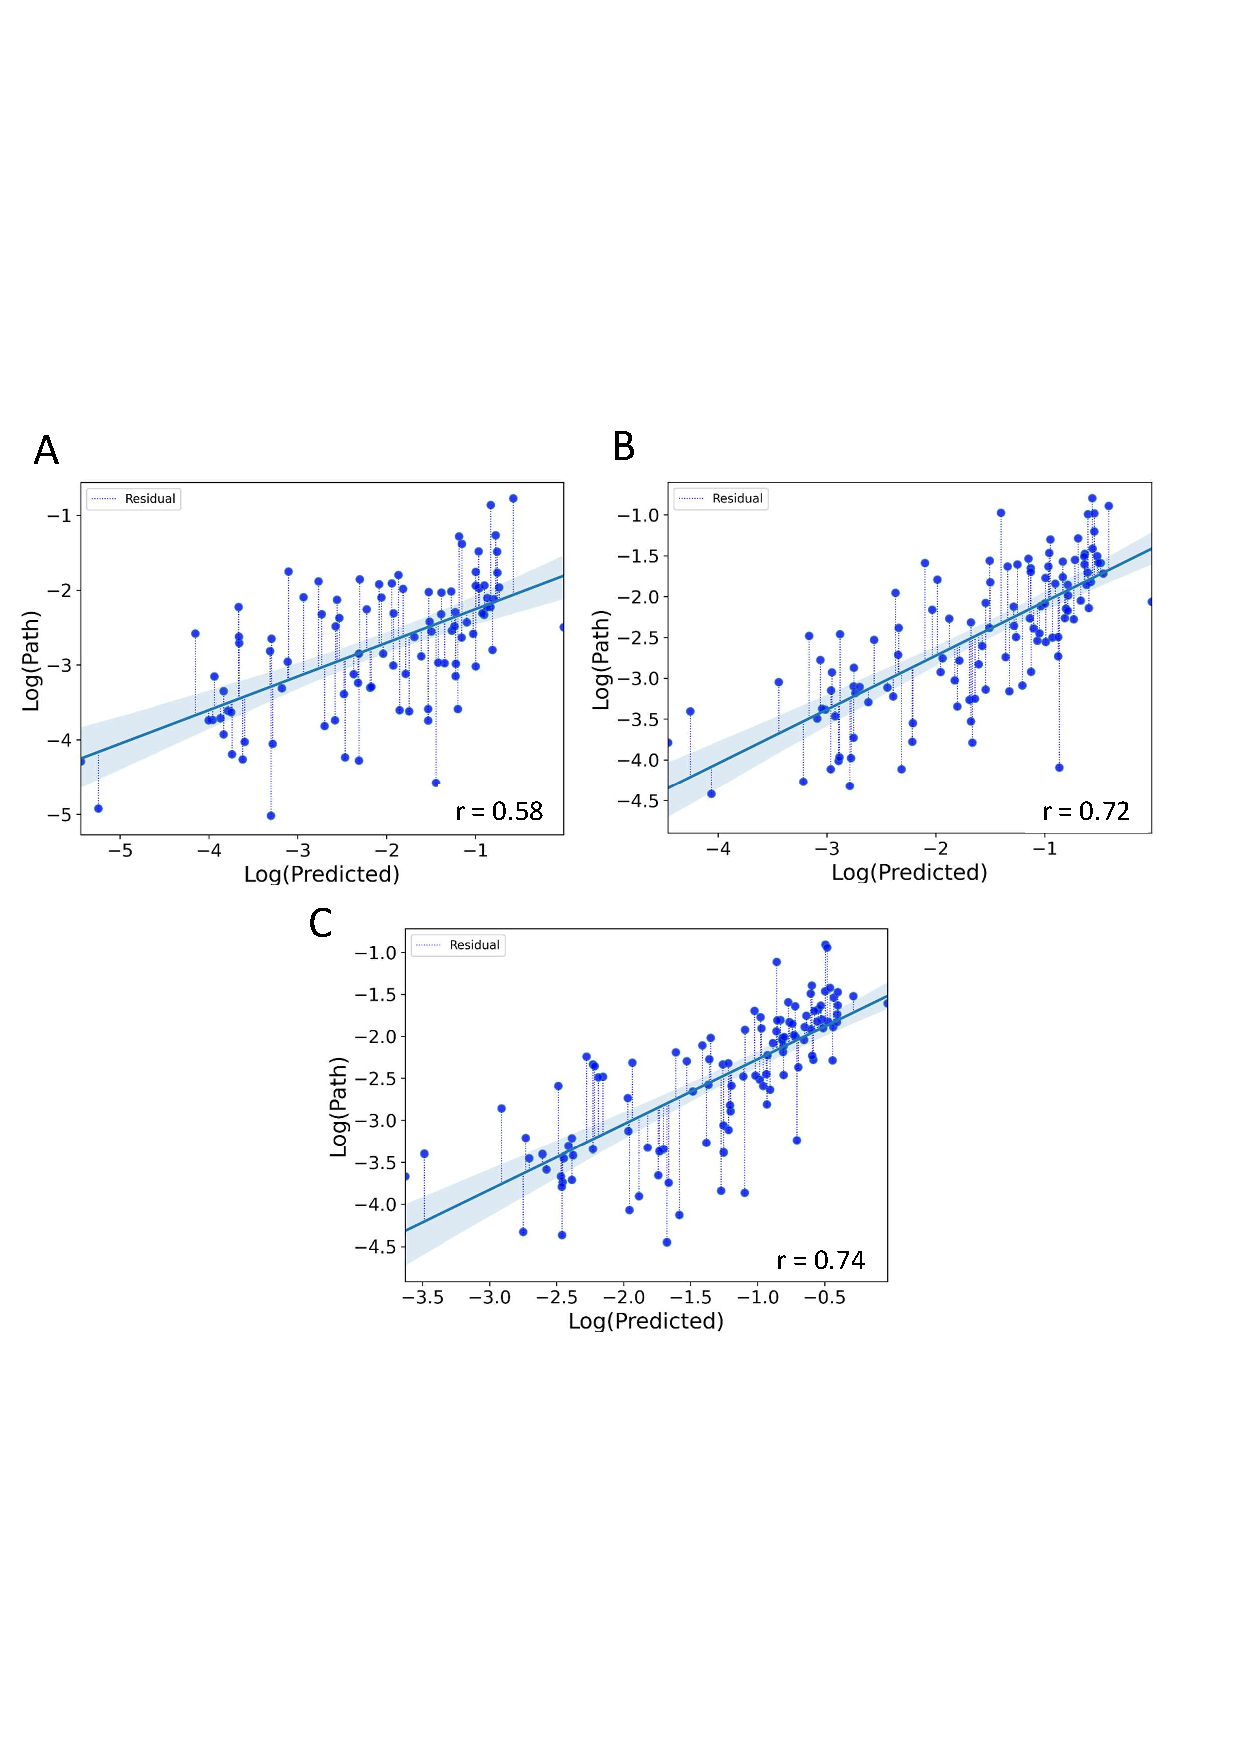
\includegraphics[width=\linewidth]{Figures/Fig3.pdf}
    \centering
    \caption{\textbf{Incorporating \textit{Snca} expression in the Diffusion Network Model improved the prediction} \\
    Scatterplots and Pearson's correlation coefficient (r) of log(predicted) pathology based on anatomical connectivity versus actual log(pathology) values when incorporating \textit{Snca} expression. Predictions versus pathology are shown after injection of PFF into the ipsilateral CPu for each region at a different timepoint.}
    \label{fig:fig3}

    \end{figure}

\subsection{\textit{In silico} seeding of alternative regions}
To examine the generalizability of the model, Henderson et al. proceeded to \textit{in silico} seeding of alternative regions such as the Piriform Cortex (Pir) and the Substantia Nigra (SN). \textbf{Figure~\ref{fig:fig4}} display the pathology spread at the MPI 1, the MPI 3 and the MPI 6 after seeding the model with either the Pir or the SN. We successfully obtained the same data sets of predictions after seeding in either the Pir or the SN. \textit{In silico} injection in the Pir remarkably corresponds to previous semi-quantitative pathology grading study as mentioned by Henderson et al. \cite{Rey_2016} While on the other hand, \textit{in silico} injection in the SN resulted in slow propagation through the Caudoputamen to cortical region as observed in the staging of human cases. Taken all together, these findings support the ability of the Diffusion Network model to generalize data predictions.

\begin{figure}
    
    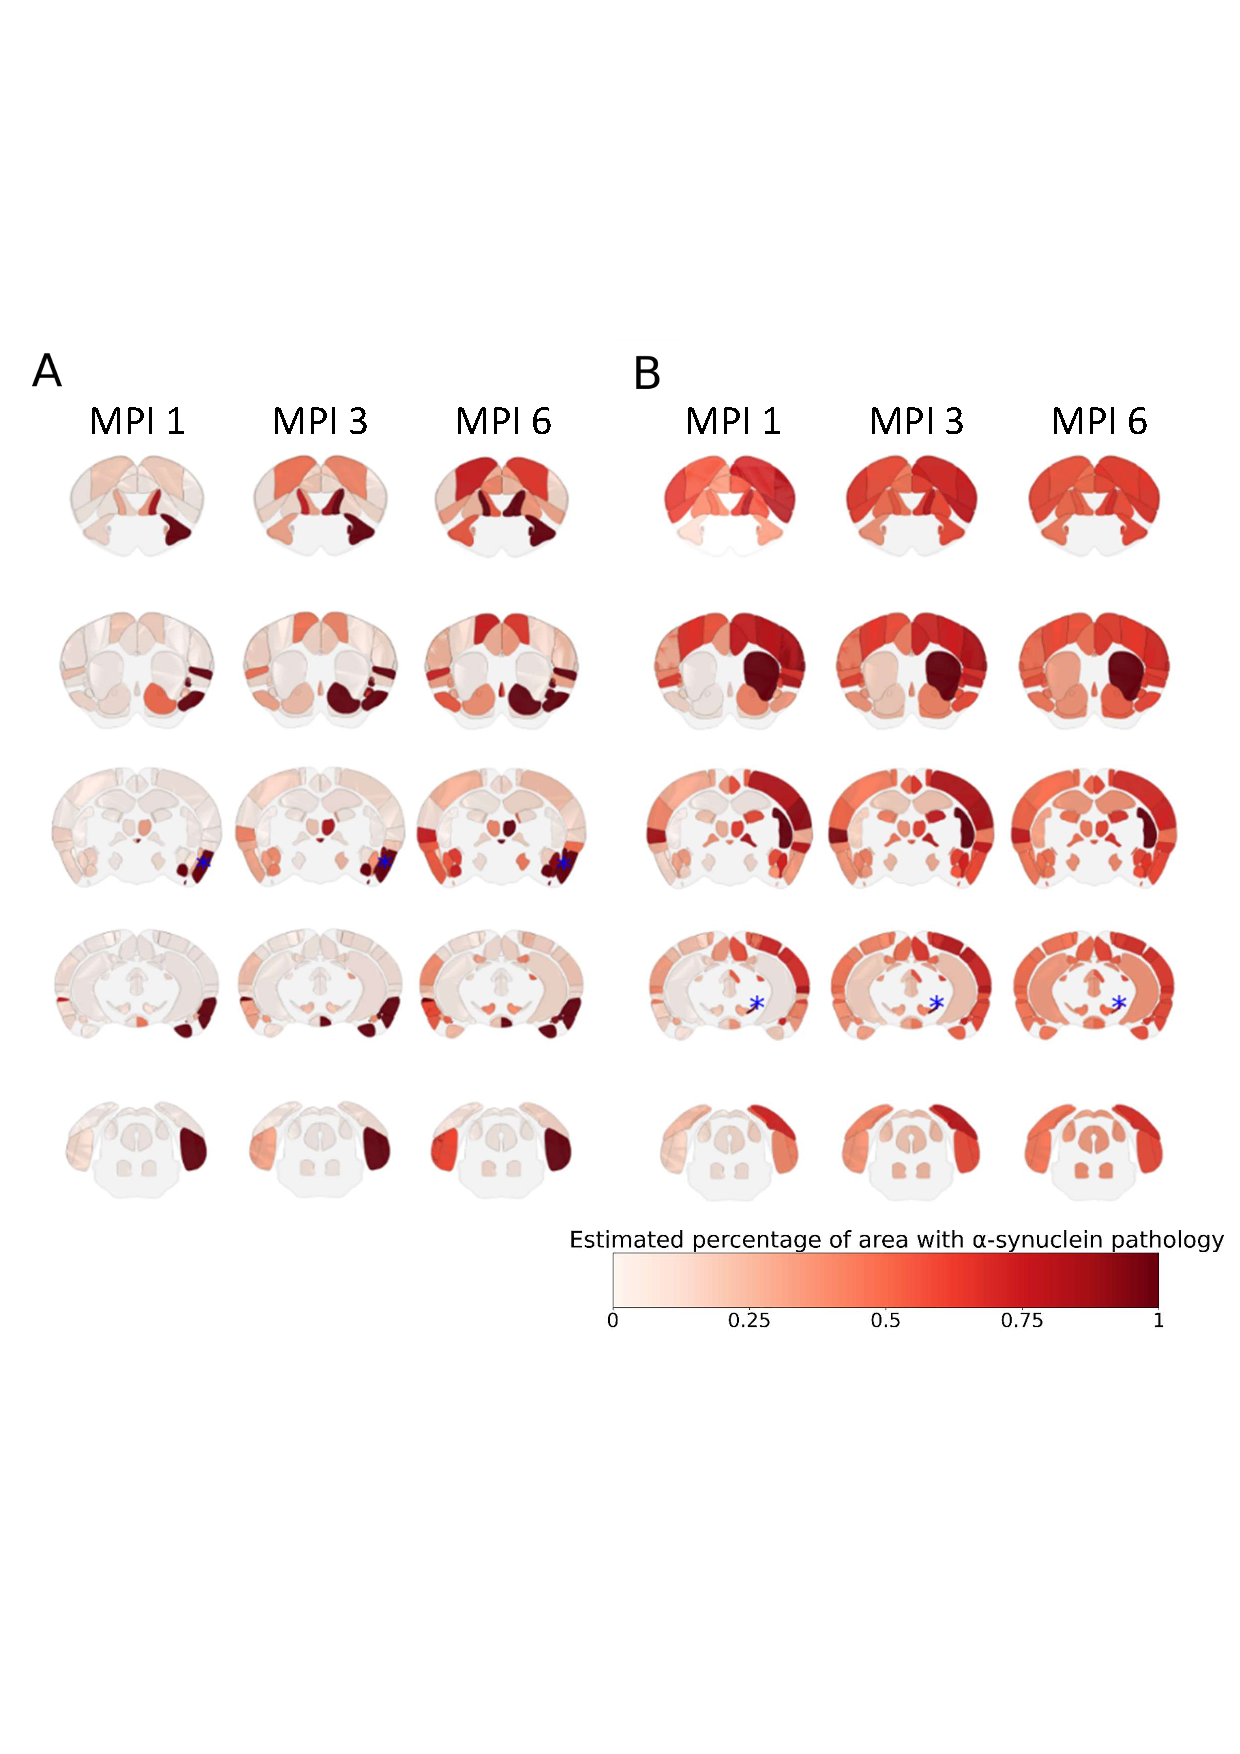
\includegraphics[width=\linewidth]{Figures/Fig4.pdf}

    \caption{\textbf{\textit{In silico} seeding of alternative regions in the mouse brain} \\
    Heat maps of regions affected by $\alpha$-synuclein pathology.
    Estimated percentage of area with $\alpha$-synuclein pathology after \textit{in silico} seeding in the Piriform Cortex (\textbf{A}) or the Substantia Nigra (\textbf{B}) The injection site is indicated on each slice by a blue asterisk. Both Figure A and B are displayed using the Python package \textit{Brainrender}. \cite{Claudi_2021}}
    \label{fig:fig4}
    \end{figure}
    

\section{Conclusion}
In this article, we successfully replicated the model created by Henderson et al. using Python.\\
\\
The Network Diffusion Model developed by Henderson et al. is a powerful tool in understanding the spread of $\alpha$-synuclein pathology. This NDM utilizes two factors: anatomical connectivity and endogenous $\alpha$-synuclein expression. Prediction of $\alpha$-synuclein spread over time has revealed islands of vulnerable neurons susceptible to developing pathogenic protein inclusions. Similarly, \textit{Snca} gene expression showed a similar pattern to inferred vulnerability. Finally, seeding in different regions such as the Pir and the SN supports the NDM generalizability. This model is attractive as it is simple, easily handled, and replicable.\\
\\
Nonetheless, some limitations raise considerations. Indeed, future empirical data are still required. Firstly, to limit sparseness in the regions sampled. Secondly, to deeply assess the generalizability of this model. Another barrier comes from that Henderson et al. adopted a mesoscale of analysis. Their observation of a distinct laminar distribution of the pathology in cortical regions suggests that further investigation should provide data about layer and neuron types affected by the disease.\\
\\
Interestingly, other models predicting pathology spread exist such as the Spatial Diffusion Model \cite{Mezias_2020} or the Epidemic Spreading Model. \cite{Vogel_2020} In their article from 2020, Henderson et al. took it even further by applying a multiple linear regression on the NDM to propose a model that examines both retrograde and anterograde contributions to the disease. \cite{Henderson_2020_tau}\\
\\
Modeling disease spread in the brain is challenging. As one could try to simulate a specific aspect, but no one would be able to simulate the brain in its entirety. Raj et al. mentioned in their review that the brain can change according to two processes that they named the "Dynamics On Network" and the "Dynamics Of Network". The first one is related to processes that occur atop a static structure as for instance prion spreading. The second defines the brain network changes over time. Parkinson's Disease exhibits dynamics in both "on" and "of" network. \cite{Raj_2018} Then, a major challenge in modeling such dynamics remains in discovering both these "on" and "of" aspects. If we were only to understand one dynamic and leave the other dynamic unexplored, we could imagine to still be a step away from the reality of the pathology.
